% latexmk -cd -lualatex -outdir=../final front_matter/general_preface.tex
% latexmk -c -outdir=final front_matter/general_preface.tex

\documentclass{ees}

\newgeometry{twoside=false,left=20mm,right=40mm,top=20mm,bottom=40mm}

\newlist{bulletlist}{itemize}{1}
\setlist[bulletlist]{
  partopsep=0pt,
  parsep=0pt,
  itemsep=0pt,
  label=\textbullet
}

\setcounter{tocdepth}{1}
\DeclareTOCStyleEntry[
  indent=0pt,
  beforeskip=\baselineskip,
  entrynumberformat=\@gobble,
  entryformat=\sbseries,
  numwidth=2em,
  linefill=\hfill,
  pagenumberbox=\pnumbox,
  pagenumberformat=\sbseries
]{tocline}{chapter}


\begin{document}

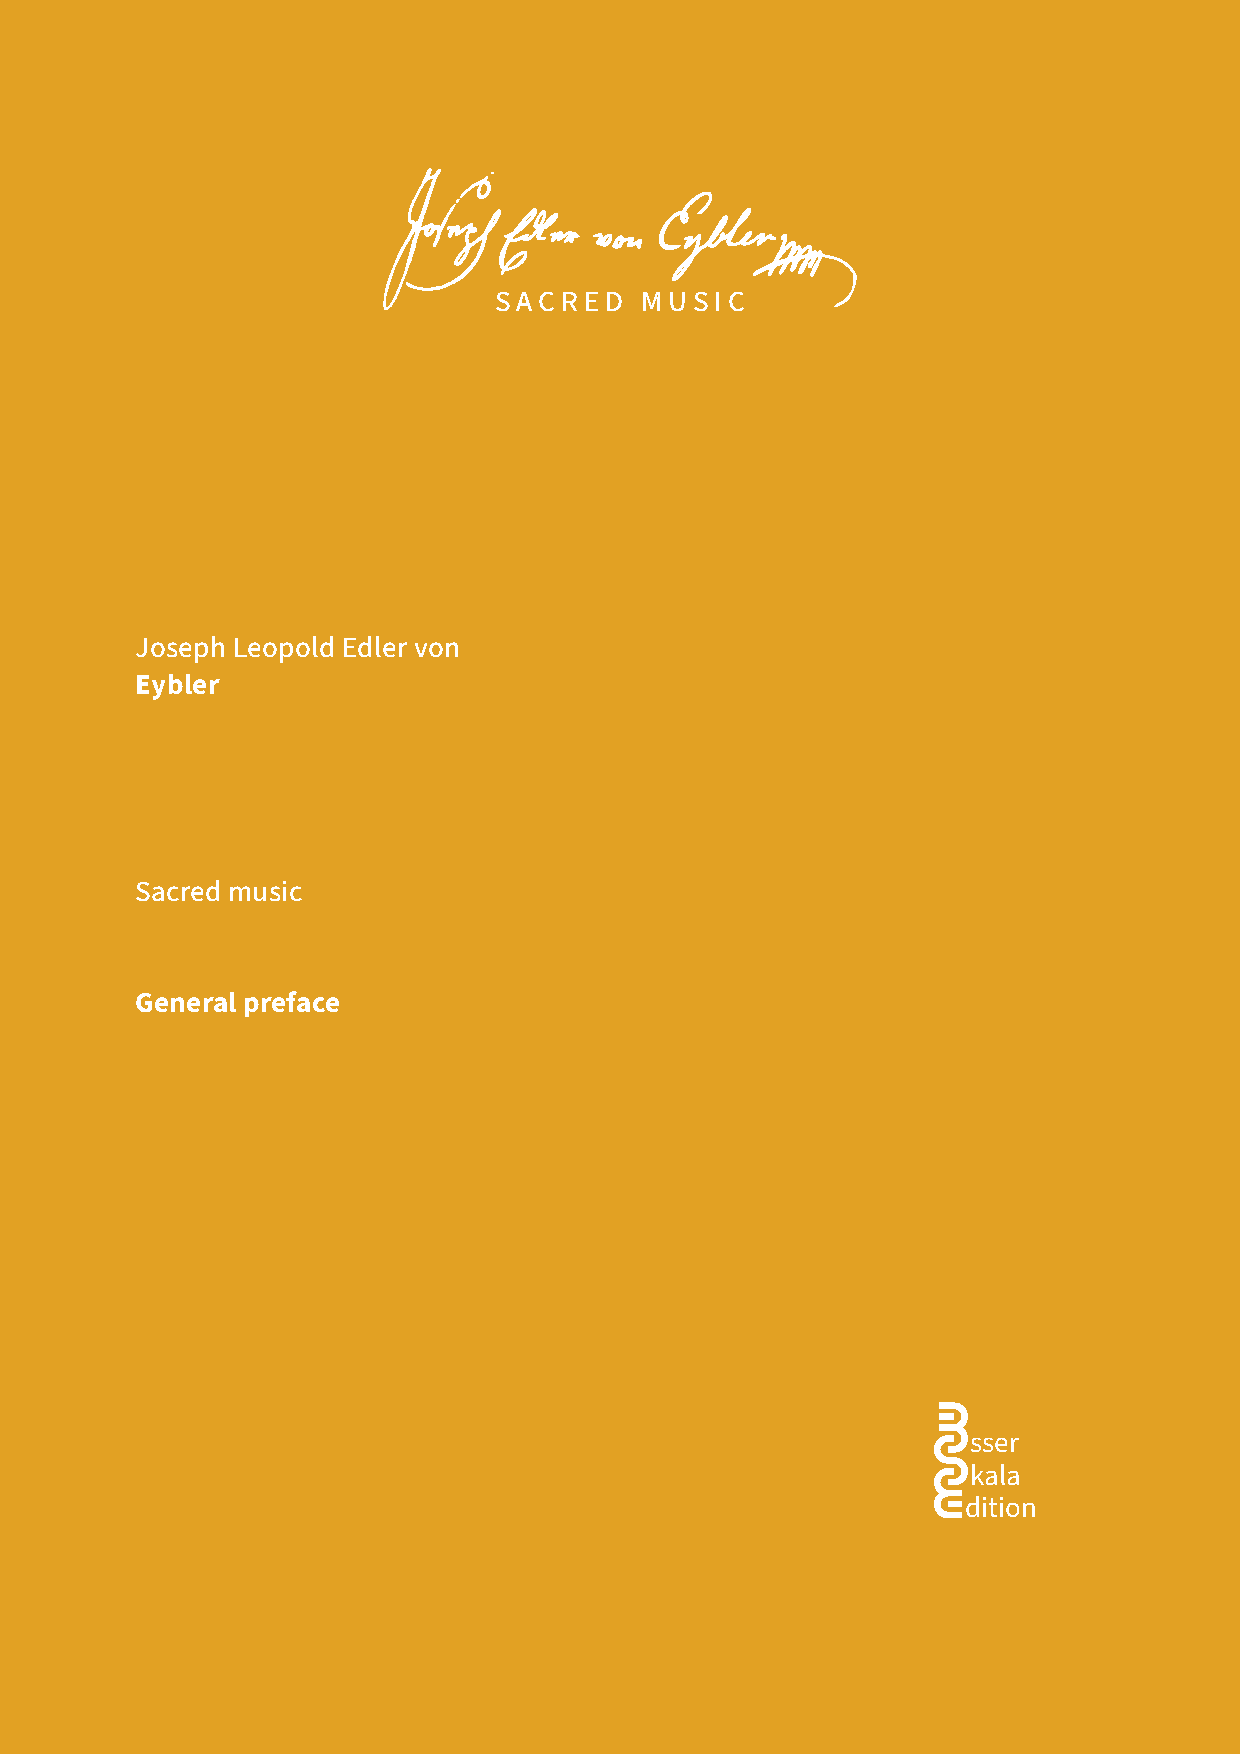
\includepdf{cover_general_preface.pdf}
\pagenumbering{arabic}
\setcounter{page}{1}

\tableofcontents

\chapter{General preface}

\textit{Joseph Leopold Edler von Eybler: Sacred Music} (JLE:SM) is an edition project that will ultimately make all of Eybler’s church music works available in modern editions.


\section{Biography}

Joseph Eybler was born on 8 February 1765 in Schwechat as the fifth of six children of the local choirmaster and school teacher. He received his first music lessons at an early age from his father, a childhood friend of Michael Haydn, and at the age of six he impressed the court official Joseph Seitz so much at a piano concert that he got him a place at the Vienna city seminary of St. Stephan. In this seminar he was taught singing, playing instruments and basso continuo. He also received composition lessons from Johann Georg Albrechtsberger from 1777 to 1779.

After the seminary was closed under Joseph II in 1782, Eybler began studying law, but soon had to give it up and earn his living as a musician. He received support from, among others, his distant relative Joseph Haydn, with whom he was friends and who recommended his compositions for publication. He also developed a close friendship with Mozart, who entrusted him with choir and soloist rehearsals for the opera \textit{Così fan tutte}. However, the bad experiences there convinced Eybler to devote himself entirely to church and chamber music after his only opera \textit{Das Zauberschwert} (1790). After Mozart's early death, Eybler was commissioned by his widow Constanze to complete the Requiem, but Eybler ultimately found himself unable to do so.

From 1792, Eybler succeeded Albrechtsberger as choir director of the Carmelites, and from 1794 to 1824 also at the Schottenstift. Through several house concerts for the imperial family, Eybler won the favor of Empress Maria Theresa, so that in 1801/1802 he was appointed imperial teacher of music and had to teach the archdukes and archduchesses. In 1803, he composed his double-choir \textit{Requiem in C minor} on commission from the Empress. In 1804 he was appointed vice-court conductor under Antonio Salieri. In 1806, Eybler married the Empress's valet, Theresia Müller; one of their two children died at the age of two. The oratorio \textit{Die vier letzten Dinge} was commissioned by the Emperor in 1810 (its libretto of which was originally intended for Joseph Haydn).

When Salieri became seriously ill in 1823, Eybler took over the direction of the court music. After Salieri's retirement, he was officially appointed the first court conductor on 6 June 1824, and thus led the court music ensemble, which consisted of around 50 orchestra musicians and choir singers. During a Mozart requiem in February 1833, Eybler suffered a stroke, which forced him to withdraw further and further from the court music. Eybler's elevation to the nobility, which had long been requested, finally took place in 1835. On 24 July 1846, Eybler passed away in the Schottenhof in Vienna and was buried in Außer-Währing, but his remains were later transferred to Schwechat.

Eybler's musical style, which shows a thorough knowledge of composition, is primarily influenced by courtly tradition and by the elder masters such as Mozart or the Haydn brothers. The vocal parts are relatively simple, but the orchestral parts are often technically demanding, with all instruments being given equal status. Eybler's work and talent were highly appreciated during his lifetime, which is reflected not least in numerous extremely positive recommendations, including from Haydn, Mozart and Albrechtsberger. Despite his great fame, Eybler was increasingly forgotten over time.


\section{Scope}

Eybler's sacred music comprises
\begin{bulletlist}
  \item masses (HerEy 1–33)
  \item mass parts (HerEy 34–36)
  \item a requiem (HerEy 37)
  \item graduals (HerEy 38–75)
  \item offertories (HerEy 76–109)
  \item marian antiphons (HerEy 110–113)
  \item te deums (HerEy 114–120)
  \item miscellaneous works (HerEy 121–136)
\end{bulletlist}

Of these works, the following will not be edited:
\begin{bulletlist}
  \item \textit{Missa Sancti Alberti} (HerEy 6) – available from \href{https://www.carus-verlag.com/musiknoten-und-aufnahmen/eybler-missa-sancti-alberti-2708400.html}{Carus}
  \item \textit{Requiem} (HerEy 37) – available from \href{https://www.kunzelmann.ch/en/requiem-oct-10287}{Edition Kunzelmann}
  \item \textit{Ecce sacerdos} (HerEy 48) – a derivative of \textit{Nocte surgentes} (HerEy 47) with different text
  \item \textit{Cantate Domino} (HerEy 66) – wrong attribution, actually by Michael Haydn (MH 828)
  \item \textit{Audite vocem magnam} (HerEy 82) – wrong attribution, actually by Antonio Salieri
  \item \textit{Domine Deus} (HerEy 101) – wrong attribution, actually by Michael Haydn (MH 827)
  \item \textit{Alleluia} (HerEy 122) – second movement of \textit{Quem tuus amor ebriat} (HerEy 38)
  \item \textit{Ad astra o mortales} (HerEy deest; A-Ws F26/6) – wrong attribution, actually by Johann Baptist Wanhal (WeiV 17b.28)
\end{bulletlist}


\section{Sources}

Most of Eybler's autographs are kept in the Schottenstift Abbey Archive; some can also be found in the Austrian National Library and in the Vienna City Library. The most important copies are the original performance materials of the Hofmusikkapelle (kept in the National Library). The following works were published during Eybler's lifetime by Tobias Haslinger:

\begin{xltabular}{\linewidth}{lrcrrX}
  \toprule
  & & & \multicolumn{2}{c}{\itshape plate number} \\
  \cmidrule{4-5}
  \itshape title & \itshape HerEy & \itshape year & \itshape full score & \itshape parts & \itshape notes \\
  \midrule \endhead
  Fremit mare & 93 & 1814 & – & 2137 \\
  Requiem & 37 & 1825 & 4701 & [4704] & parts never printed \\
  Missa Sanctorum Apostolorum & 15 & 1826 & 4791 & 4794 & 1. Messe \\
  Tua est potentia & 50 & 1826 & 4792 & 4795 & 1. Graduale \\
  Domine si observaveris & 88 & 1826 & 4793 & 4796 & 1. Offertorium \\
  Missa Sancti Mauritii & 4 & 1827 & 5011 & 5014 & 2. Messe \\
  Sperate in Deo & 41 & 1827 & 5012 & 5015 & 2. Graduale \\
  Si consistant & 86 & 1827 & 5013 & 5016 & 2. Offertorium \\
  Missa Sancti Leopoldi & 12 & 1827 & 5045 & 5048 & 3. Messe \\
  Omnes de saba & 40 & 1827 & 5046 & 5049 & 3. Graduale \\
  Reges Tharsis & 107 & 1827 & 5047 & 5050 & 3. Offertorium \\
  Missa Sancti Ludovici & 3 & 1829 & 5243 & 5246 & 4. Messe\\
  Dies sanctificatus & 61 & 1829 & 5244 & 5247 & 4. Graduale \\
  Tui sunt coeli & 78 & 1829 & 5245 & 5248 & 4. Offertorium \\
  Missa Sancti Josephi/Rudolphi & 17 & 1829 & 5427 & 5430 & 5. Messe \\
  Benedicamus Patrem & 55 & 1829 & 5428 & 5431 & 5. Graduale \\
  Iubilate Deo & 91 & 1829 & 5429 & 5432 & 5. Offertorium \\
  Missa Sancti Raineri & 20 & 1831 & 5559 & 5562 & 6. Messe \\
  Non in multitudine & 56 & 1831 & 5560 & 5563 & 6. Graduale \\
  Timebunt gentes & 87 & 1831 & 5561 & 5564 & 6. Offertorium \\
  Missa coronationis Ferdinandi & 5 & 1832 & 5740 & 5743 & 7. Messe \\
  Domine Deus omnium creator & 42 & 1832 & 5741 & 5744 & 7. Graduale \\
  Magna et mirabilia & 108 & 1832 & 5742 & 5745 & 7. Offertorium \\
  \bottomrule
\end{xltabular}


\section{Prior editions}

\begin{bulletlist}
  \item \href{https://www.doblinger.at/shop/okm-00005-st-dies-sanctificatus-tui-sunt-coeli-170430}{\textit{Dies sanctificatus}} (HerEy 61) and \textit{Tui sunt coeli} (HerEy 78) edited by Karl Pfannhauser (Doblinger)
  \item \href{https://boehm-und-sohn.de/produkt/jubilate-deo-4}{\textit{Iubilate Deo}} (HerEy 91) edited by Felix Schroeder (Böhm \& Sohn)
  \item \href{https://boehm-und-sohn.de/produkt/omnes-de-saba}{\textit{Omnes de Saba}} (HerEy 40) and \href{https://boehm-und-sohn.de/produkt/terra-tremuit}{\textit{Terra tremuit}} (HerEy 85) edited by Rouland Carl (Böhm \& Sohn)
  \item \href{https://www.carus-verlag.com/musiknoten-und-aufnahmen/eybler-missa-sancti-alberti-2708400.html}{\textit{Missa Sancti Alberti}} (HerEy 6) edited by Armin Kircher (Carus)
  \item \href{https://www.kunzelmann.ch/en/requiem-oct-10287}{\textit{Requiem}} (HerEy 37) edited by Franz Beyer (Edition Kunzelmann)
  \item three masses, as well as several graduals and offertories edited by Manfred Hößl (available at \href{https://www.cpdl.org/wiki/index.php/Josef_von_Eybler}{CPDL})
  \item \textit{Omnes de Saba} (HerEy 40), \textit{Sperate in Deo} (HerEy 41), \textit{Domine Deus} (HerEy 42), \textit{Tristes erant Apostoli} (HerEy 123), \textit{Iste Confessor} (HerEy 124), and \textit{Ecce quomodo moritur} (HerEy 125) edited by Reinhold Kainhofer (\href{https://edition-kainhofer.com}{Edition Kainhofer})
\end{bulletlist}


\section{Eybler's autograph catalogue of works}

The Schottenstift Abbey archive holds an incomplete catalogue of works assembled by Eybler himself (siglum Cod. 707/1). This catalogue consists of two oblong bifolios, containing 16 staves per page.
\begin{bulletlist}
  \item fol. 1: [above first staff, centered, in ink] Catalogo della musica sacra. [below: descriptions of Te Deums 1–7 and masses 1–11]
  \item fol. 2: [masses 12–16, offertories 1–13]
  \item fol. 3: [offertories 14–23]
  \item fol. 4: [graduals 1–16]
  \item fol. 5: [graduals 17–30, requiem, libera]
  \item fol. 6: [masses 17–21]
  \item fol. 7: [above first staff, in pencil] Unvollſtändiger Catalog [in red pencil] 1
  \item fol. 8: [short masses 1–3]
\end{bulletlist}

These works descriptions are summarized below (incipits are omitted).{\footnotesize
\begin{xltabular}{\linewidth}{>{\itshape}rrlc X}
  \toprule
  & \itshape HerEy & \itshape title & \itshape year & \itshape notes \\
  \midrule \endhead
  & & \itshape Missæ \\
  \cmidrule(lr){3-3}
  1  &   1 & Sti Hermani & 1781 &  \\
  2  &   8 & Sti Benonis & 1797 &  \\
  3  &  11 & Sti Wolfgangi & 1800 &  \\
  4  &  29 & Stæ Theresiæ & 1802 &  \\
  5  &   2 & Sti Michaelis & 1804 &  \\
  6  &  30 & Sti Francisci & 1806 & Nb doppelchörig. \\
  7  &  17 & Sti Josephi & 1807 &  \\
  8  &  22 & Stæ Eleonoræ & 1809 &  \\
  9  &  13 & Sti Ignatii & 1816 &  \\
  10 &   9 & Sti Caroli & 1817 & [original name “Andreæ” crossed out] \\
  11 &  28 & Stæ Elisabethæ & 1818 &  \\
  12 &  18 & Sti Maximiliani & 1819 &  \\
  13 &  12 & Sti Leopoldi & 1820 &  \\
  14 &  14 & Stæ Andreæ & 1821 & [original name “Caroli” crossed out] \\
  15 &   5 & Sti Ferdinandi & 1822 &  \\
  16 &   3 & Sti Ludovici & 1823 &  \\
  17 &  15 & SS: Apostolorum & 1825 & [above name: “Coronationis \&”] \\
  18 &   4 & Sti Mauritii & 1825 &  \\
  19 &  19 & Sti Rudolphi & 1826 &  \\
  20 &  32 & Sti Antonii & 1827 &  \\
  21 &  10 & Sti Joannis & 1828 &  \\
  \midrule
  & & \itshape Missæ breviores \\
  \cmidrule(lr){3-3}
  1 & 31 & Sti Theodori & 1821 & \\
  2 & 23 & Sti Georgii & 1821 & \\
  3 & 16 & Sti Clementis & 1824 & [original date 1825 corrected to 1824] \\
  \midrule
  & & \itshape Requiem \\
  \cmidrule(lr){3-3}
    & 37 & Requiem & 1803 & Nb Dies iræ iſt doppelchörig \\
    & 37 & Libera & 1803 & Nb 7 ſtimmig mit Harmonie Begleitung. \\
  \midrule
  & & \itshape Te Deum \\
  \cmidrule(lr){3-3}
  1 & 118 & Te Deum & 1800 &  \\
  2 & 120 & Te Deum & 1802 & Nb auch 2 chörig mit vermehrter Inſtrumental Begleitung. \\
  3 & 117 & Te Deum & 1804 &  \\
  4 & 114 & Te Deum & 1807 & Nb doppelchörig \\
  5 & 115 & Te Deum & 1814 & Nb doppelchörig \\
  6 & 119 & Te Deum & [1819] &  \\
  7 & 116 & Te Deum & 1825 &  \\
  \midrule
  & & \itshape Offertoria \\
  \cmidrule(lr){3-3}
  1  &  95 & Lux est orta & 1806 & 4 ſtimmiger Canon Solo, mit Begleitung von 2 Chören. De Tempore. \\
  2  &  85 & Terra tremuit, \& quievit & 1797 & de Resurrectione Domini \\
  3  &  96 & Ad te, o summa bonitas & 1816 & Tenore, \& Clarinetto Concti con Coro Acc: de Tempore \\
  4  & 100 & O Maria Virgo pia & 1815 & 4 ſtimmiger Canon Solo, mit zulezt Coro tutto, de B: V: M: \\
  5  &  93 & Fremit mare cum furore & 1800 & in der Mitte mit Soprano und Clarinetto Solo, de Tempore \\
  6  & 104 & Levavi in montes oculos meos & 1802 & per 2 Soprani Concti, e Coro ripieno, de Tempore \\
  7  &  98 & Ad te levavi animam meam & 1804 & Soprano Solo e Coro ripieno, de Tempore \\
  8  & 107 & Reges Tharsis […] & 1807 & Tutti, de Epiphania Domini \\
  9  &  43/86 & Si consistant adversum me castra & 1805 & in der Mitte Solo Geſang mit 4 Männer Stimmen und Harmonie, de Tempore \\
  10 &  97 & Levavi in montes & 1818 & Baſso \& Clarinetto Solo mit Coro Begleitung, de Tempore \\
  11 &  92 & Laus sit Deo, in excelsis & 1794 & Tutti, de Nativitate Domini, oder de Tempore [original date 1795 corrected to 1974; in pencil: “nicht vorhanden”] \\
  12 & 106 & Laudate pueri Dominum & 1802 & de Tempore \\
  13 & 132 & De profundis clamavi ad te & 1803 & de Tempore \\
  14 &  90 & Summe Deus & 1818 & Tenore, Violino \& Violoncello Solo mit Coro Begleitung, de Tempore \\
  15 &  38 & Quem tuus amor ebriat & 1797 & Alto Solo, Alleluja mit Chor Begleitung, de Tempore \\
  16 &  83 & Surrexit vere tumolo Redemptor & 1794 & Baſso Solo, de Resurrectione Domini [in pencil: “nicht vorhanden”] \\
  17 &  91 & Jubilate Deo omnis terra & 1820 & Tutti, de Tempore \\
  18 &  88 & Domine si observaveris & 1821 & Soprano Solo mit Coro Begleitung, de Tempore \\
  19 &  76 & Nos populus tuus & 1822 & Tutti, de tempore \\
  20 &  77 & Jubilate Deo universa terra & 1823 & Tutti, e con tutti gli Stromenti, de Tempore \\
  21 &  79 & Confirma hoc Deus & 1825 & Tutti, in Festo Pentecostes ò de Spiritu Sancto \\
  22 &  78 & Tui sunt cœli & 1827 & Tutti, in Festo SS: Nativitatis D: N: J: C: in 3tia Miſsa \\
  23 & 108 & Magna \& mirabilia & 1828 & Tutti, de Tempore \\
  \midrule
  & & \itshape Gradualia \\
  \cmidrule(lr){3-3}
  1  &  68 & Exaltate Dominum […] & 1806 & Nb doppelchörig, Tutti, de Tempore\\
  2  &  70 & Justus ut palma florebit & 1807 & Tutti, de Confeſsore\\
  3  &  69 & Iste est, qui ante Deum & 1807 & Tutti, de Confeſsore\\
  4  &  53 & Specie tua & 1796 & Tutti, de quævis Sancta\\
  5  &  54 & Christus factus est & 1797 & Tutti, in Cœna Domini\\
  6  &  87 & Timebunt gentes […] & 1817 & Tutti de Tempore, Nb doppelchörig, Nb iſt Offertorium\\
  7  &  58 & Victimæ paschali laudes […] & 1817 & de Resurrectione Domini\\
  8  & 121 & Veni Sancte Spiritus & 1818 & de Festo Pentecostes\\
  9  &  47 & Nocte Surgentes & 1800 & Tutti, de Tempore\\
  10 &  67 & Magnificate Dominum meum & 1802 & Tutti con Clarino Concto, de Tempore\\
  11 &  39 & Cantate Domino & 1804 & Tutti, de Tempore\\
  12 &  40 & Omnes de Saba venient & 1807 & de Epiphania Domini\\
  13 &  49 & Te Summe Jesu & 1809 & Tutti, de SS: Nomine Jesu, aut de Tempore\\
  14 &  46 & Os Justi meditabitur sapientiam & 1805 & Tutti, de Confeſsore\\
  15 &  65 & Ave Maria, gratia plena & 1819 & Tutti, de B: V: M:\\
  16 &  57 & Alma Redemptoris Mater & 1815 & Tutti, de B: V: M: tempore, Adventus, \& Nativitatis Domini\\
  17 & 113 & Salve Regina & 1809 & Tutti, de B: V: M:, post tempus paschale\\
  18 & 111 & Regina cœli lætare & 1817 & Tutti, de B: V: M:\\
  19 &  71 & Ave Regina & 1819 & Soprano Concto e Coro Ripieno de B: V: M:, tempore Quadragesmiæ\\
  20 &   – & Benedicam Dominum in omni tempore & 1820 & Tutti de Tempore\\
  21 &  50 & Tua est potentia & 1822 & Tutti de Tempore\\
  22 &  41 & Sperate in Deo & 1822 & Tutti de Tempore, Nb Oboe solo\\
  23 &  56 & Non in multitudine & 1823 & Tutti de Tempore\\
  24 & 110 & Regina cœli lætare & 1825 & Tutti, e con tutti gli Stromenti de B: V: M:, tempore paschali\\
  25 &  59 & Beata gens & 1825 & Sto Spiritu, ò in Festo Pentecostes\\
  26 &  42 & Domine Deus, omnium creator & 1826 & Tutti de Tempore\\
  27 &  60 & Peccata dimittis & 1826 & Tutti de Tempore\\
  28 &  61 & Dies sanctificatus & 1827 & Tutti de Festo SS: Nativitatis D: N: J: Co in 3tia Miſsa\\
  29 &  44 & Per te Dei Genitrix & 1828 & Tutti de B: V: M:\\
  30 & 125 & Ecce quomodo moritur justus & 1816 & a 4tro, mit 3 Poſaunen bey der Grablegung des Herrn \\
  \bottomrule
\end{xltabular}}


\section{Editorial guidelines}

In general, JLE:SM follows the \href{https://edition.esser-skala.at/about/editorial-guidelines/}{editorial guidelines} for the Edition Esser-Skala. Some peculiarities for editing Eybler's works are highlighted below:

\begin{bulletlist}
  \item The viola staff is – as in most autograph scores – titled “Viole” (plural).
  \item For the same reason, the bass group staff is titled “Organo, Violoncello e Bassi”.
  \item Eybler's bass figures occasionally contain the figure 5 with a roof. This figure indicates a diminished triad that should not be played as a sixth-fifth chord.
  \item If there are many differences between violone and organ, they are notated on two staffs in the full score.
  \item In the timpani, trill spans on a single note are converted to trill signs.
  \item In the autographs, where there are several instruments per staff, a separate clef is written for each instrument at the beginning of the staff. Here, only a single clef is printed.
  \item In the autographs, slurs are sometimes placed over notes where there are no melismas. Here, slurs are placed as dictated by the syllable allocation (which is more familiar to singers).
  \item Eybler uses “Tutti” and “Solo” in the bass staff also to indicate forte and piano sections of the chorus. This practice is retained here.
  \item In the autographs, bass figures are generally absent in sections that are marked as “Solo”, likely indicating that the organ should not play chords. Here, bass figures have nevertheless been added in these sections.
  \item The directive “Solo” in instrumental parts is generally not reproduced here.
\end{bulletlist}

\clearpage
\section{Printed editions}

Works in JLE:SM will also appear in print at Amazon Kindle Direct Publishing. Currently, the following volumes are available:

\begin{xltabular}{\linewidth}{rllrX}
  \toprule
  & & & \multicolumn{2}{l}{\itshape contents} \\
  \cmidrule(lr){4-5}
  \itshape volume & \itshape published & \itshape ASIN & \itshape HerEy & \itshape title \\
  \midrule \endhead
  \itshape Series A & \multicolumn{2}{l}{\itshape Masses} \\*
  \cmidrule(lr){1-3}
  1 & 2024-07 & \href{https://www.amazon.de/dp/B0D8HQRNT4}{B0D8HQRNT4}
                           & 11 & Missa Sancti Wolfgangi \\
  \midrule
  \itshape Series B & \multicolumn{2}{l}{\itshape Short liturgical works} \\*
  \cmidrule(lr){1-3}
  1 & 2024-07 & \href{https://www.amazon.de/dp/B0D973PCYF}{B0D973PCYF}
                           & 44    & Per te Dei genitrix \\
    &         &            & 47    & Nocte surgentes \\
    &         &            & 50    & Tua est potentia \\
    &         &            & 53    & Specie tua \\
    &         &            & 54    & Christus factus est \\
    &         &            & 56    & Non in multitudine \\
    &         &            & 61    & Dies sanctificatus \\
    &         &            & 78    & Tui sunt cœli \\
    &         &            & 85    & Terra tremuit \\
    &         &            & 86/43 & Si consistant \\
    &         &            & 93    & Fremit mare cum furore \\
    &         &            & 107   & Reges Tharsis \\
    &         &            & 132   & De profundis \\
  \bottomrule
\end{xltabular}


\section{Acknowledgements}

Permission of the Schottenstift Abbey Archive to use their archival materials for this edition is gratefully acknowledged. We thank Dr. Maximilian Alexander Trofaier for assistance in obtaining these documents; the staff of the Austrian National Library and the Vienna City Library for support; and Dr. Reinhold Kainhofer for his previous work on the Eybler Edition.


\section{Bibliography}

\begin{bulletlist}
  \item Badura-Skoda, Eva, and Herrmann-Schneider, Hildegard (2001). Eybler, Joseph [Josef] Leopold, Edler von. \href{https://doi.org/10.1093/gmo/9781561592630.article.40047}{Grove Music Online}.
  \item Boisits, Barbara, and Haas, Robert (2016). Eybler, Joseph Leopold Edler von. \href{https://www.mgg-online.com/mgg/stable/13179}{MGG Online}.
  \item Eybler, Joseph Leopold (n.d.). Catalogo della musica sacra. Manuscript, A-Ws Cod. 707/1.
  \item Herrmann, Hildegard (1976). Thematisches Verzeichnis der Werke von Joseph Eybler. Musikverlag Emil Katzbichler, München–Salzburg.
  \item Ölsinger, Franz (1932). Die kirchenmusikalischen Werke Joseph Eyblers. PhD thesis, University of Vienna.
  \item Weinmann, Alexander (1979–1983). Vollständiges Verlagsverzeichnis Senefelder Steiner Haslinger. 3 vols. Musikverlag Emil Katzbichler, München–Salzburg.
\end{bulletlist}

\clearpage
\markdownInput{../CHANGELOG.md}

\end{document}
